\chapter{Suivi de trajectoire}
\label{chap:suivi}

\epigraph{Text text text text text text text text text text text text
  text text text text text text text text text text text text text
  text text text text text text text text text text text text text
  text text text text text text text text text text text text text
  text text text text}{Some Author}
\clearpage

\lettrine[lines=2, lraise=0.1, nindent=0em, slope=-.5em]%
{C}{e} chapitre est dédié au problème de la génération et de
l'exécution asservie de trajetoires pour un robot humanoïde. Les
robots humanoïdes sont des robots aillant une forme anthropomorphique:
une tête, deux bras, deux jambes et un torse. La locomotion est donc
bipède et les robots humanoïdes ont la possibilité d'effectuer des
tâches dextres. De ces choix résultent un système hautement dimensioné
pour lequel il est difficile de générer des trajectoires et dont le
contrôle est délicat, l'équilibre d'un système bipède étant précaire
par nature. Au long de ce chapitre, nous verrons comment modéliser ce
système, comment représenter et calculer des mouvements pour ce
dernier afin qu'il puisse se mouvoir et réaliser différentes
tâches. Serons ensuite étudiée les différentes approches de la
littérature ainsi que leurs forces et leurs faiblesses. La troisième
section portera sur l'apport de cette thèse au problème de l'exécution
de trajectoire via la proposition d'une architecture de contrôle pour
les robots humanoïdes asservie capteur. Les résultats expérimentaux
seront ensuite détaillés pour illustrer une tâche dans laquelle le
système proposé se révèle utile. Enfin, les prospectives montreront
quelles sont les possibilités d'améliorations de l'approche proposée
et quels futurs travaux restent à réaliser.

\section{Génération de mouvements pour les robots humanoïdes}
\subsection{Structure robotique}

Un robot est un système composé par des actionneurs -- moteurs --, des
capteurs et des unités de calcul logique -- ordinateurs -- travaillant
de concert pour constituer une entité cohérente pouvant impacter le
monde réel afin de réaliser l'objectif qui lui a été confié. En ce qui
concerne la génération de l'exécution de mouvements, deux éléments
sont primordiaux: d'une part les capacités motrices du système,
modélisés sous la forme d'un arbre cinématique et d'autre part sa
forme dans le monde représentée par la forme géométrique des
différentes partie du système. La forme géométrique d'un robot variant
généralement sous l'action de ses actionneurs, elle est donc
conditionée par l'état de l'arbre cinématique.

\begin{mydef}
  Un arbre cinématique est un ensemble de joints formant un arbre.
  Soit $\mathcal{A}$ un arbre cinématique, on a:

  \begin{equation}
    \mathcal{A} = \emptyset \cup \{ (\mathcal{J}_0, \mathcal{C}_0),
    \dotsc, (\mathcal{J}_n, \mathcal{C}_n) \}
  \end{equation}

  Un arbre est donc soit l'ensemble vide soit une liste de joints
  associé à un sous-arbre. Cette définition permet de construire
  récursivement un arbre cinématique.

  A cet arbre de joints correspond une liste de joints, les joints
  sont habituellement référencés par leur ordre dans cette liste sous
  la notation $\mathcal{J}_n$ où $n$ est la position du joint dans la
  liste.
\end{mydef}

\begin{mydef}
  Le joint $\mathcal{J}_n$ modélise le mouvement du repère $n+1$ par
  rapport au repère $n$ selon un certain nombre de paramètres appelés
  degrés de liberté. Chaque joint définit implicitement son repère
  attaché. Le repère attaché à $\mathcal{J}_0$ est habituellement
  appelé repère ``monde'' et est noté $\mathcal{W}$.

  Un joint peut donc se modéliser comme une fonction:

  \begin{equation}
    \left\{
    \begin{array}{cccc}
      \mathcal{J}_n : & \mathbb{R}^m & \rightarrow & SE(3)\\
      & \mathbf{q} & \mapsto & \mathcal{J}_n(t)
    \end{array}
    \right.
  \end{equation}

  Dans l'équation le joint $\mathcal{J}_n$ possède $m$ degrés de
  liberté permettant de déterminer la transformation relative entre le
  repère $n$ et $n + 1$ qui est un élément du groupe spécial euclidien
  de dimension 3. Ces fonctions permettent donc d'exprimer des
  contraintes sur les mouvements des corps du robot au niveau des
  articulations actionées.
\end{mydef}

Plusieurs types de joints sont habituellement utilisés en robotique,
mais nous n'allons ici en détailler que deux:
\begin{description}
\item[Joint libre -- ou joint flottant --] Ce joint comporte six degrés de libertés, soit le
  nombre de paramètres nécessaire et suffisant pour spécifier une pose
  dans $SE(3)$. Autrement dit, ce joint n'impose aucune contrainte
  particulière sur le mouvement et correspond donc à la fonction
  identité, à la représentation de la pose près.
\item[Joint rotation] Ce joint comporte un seul degré de liberté. Dans
  ce cas, la position du prochain corps du robot est défini par la
  valeur de ce degré de liberté, interprété comme une rotation d'un
  angle équivalent autour d'un axe. A chaque joint rotation est donc
  soit associé un axe de rotation, soit un axe standard est choisi:
  par exemple, toutes les rotations seront réalisées autour de l'axe
  X.
\end{description}


Une fois cette structure construite, un souhaite naturel est de
souhaiter pouvoir exprimer son état. C'est l'objectif du vecteur de
configuration.

\begin{mydef}
  Soit $\mathbf{q}$ le vecteur de configuration de l'arbre cinématique
  $\mathcal{C}$. Soit $\mathcal{J}_0, \dotsc, \mathcal{J}_n$
  l'ensemble des joints de $\mathcal{C}$. Le vecteur de configuration
  a pour dimension: $\sum_{i=0}^n \#\mathcal{J}_i$, la somme des arités
  des joints interprétés comme fonctions, c'est à dire la somme du
  nombre de degrés de liberté de tous les joints.


  Les valeurs du vecteur de configuration sont alors les valeurs des
  degrés de liberté des joints concaténés les uns aux autres selon un
  parcours de l'arbre donné. En général, le parcours main gauche de
  l'arbre est utilisé.
\end{mydef}

\begin{figure}[htbp!]
  \begin{center}
  \begin{tikzpicture}
    \Tree [ .{$\mathcal{J}_0$ (6)} [ .{$\mathcal{J}_1$ (1)} {$\mathcal{J}_2$ (2)} {$\mathcal{J}_3$ (1)} ] {$\mathcal{J}_4$ (1)} ]
  \end{tikzpicture}

  \begin{tabular}{|ccc|c|cc|c|c|}
    \hline
    $\mathcal{J}_0$ (1) & \ldots & $\mathcal{J}_0$ (6)
    & $\mathcal{J}_1$ (1) & $\mathcal{J}_2$ (1) & $\mathcal{J}_2$ (2) & $\mathcal{J}_3$ (1) & $\mathcal{J}_4$ (1)\\
    \hline
  \end{tabular}
  \end{center}

  \caption{Un exemple de chaîne cinématique et son vecteur de
    configuration correspondant. Les nombres entre parenthèses
    indiquent le nombre de degrés de liberté dans l'arbre ou le numéro
    du degré de liberté dans le joint pour le vecteur de
    configuration.}
\end{figure}

On notera que l'arbre cinématique d'un robot humanoïde est souvent
composé d'un joint libre à la racine suivi de joints rotation pour le
reste de l'arbre. À partir de maintenant, cette forme sera
systématiquement utilisée ce qui nous permettra de diviser le vecteur
de configuration en deux parties: d'un côté la position du robot dans
le plan, définie par une sous-partie des degrés de liberté du joint
libre à la racine, le repère de ce joint définissant de ce fait le
repère monde $\mathcal{W}$ et d'autre part les degrés de liberté
internes correspondant à une réalité méchanique. On aura donc:

\begin{equation} \label{eq:chap2_configuration}
  \begin{aligned}
    \mathbf{x} &= [x, y, r_z]\\
    \mathbf{q} &= (\mathbf{x}, [z, r_x, r_y, \mathbf{q}_{\text{int}}])
    \in \mathcal{C} = \text{SE}(2) \times \mathcal{C}_{\text{int}}
  \end{aligned}
\end{equation}

Les six paramètres du joint racine sont: $[x, y, z, r_x, r_y, r_z]$ et
définissent une position dans l'espace 3d. Toutefois, dans la mesure
où la position du robot est contrainte par la physique, c'est à dire
que l'on peut raisonnablement supposer un contact planaire entre les
pieds du robot et le sol, on peut se contenter de considérer la
position du robot en deux dimensions dans le plan. Pour cette raison,
on peut considérer: $\mathbf{x} = [x, y, r_z] \in \text{SE}(2)$ pour
déterminer la position du robot dans l'espace. $\mathcal{C}$
représente alors l'espace des configurations et
$\mathcal{C}_{\text{int}}$ est l'espace des configurations
correspondant aux degrés de liberté internes uniquement. Ce découpage
peut sembler arbitaire au premier abord mais prend son sens quand on
considère quels degrés de liberté peuvent dériver suite à des erreurs
de modélisation ou d'exécution: la position du robot dans le plan peut
s'avérer fausse et doit être estimée et corrrigée constamment alors
que les degrés de liberté $[z, r_x, r_y]$ ne peuvent pas subir de
dérives durant le mouvement. Le problème de la correction des erreurs
est détaillé plus loin dans ce chapitre et le problème de la
localisation d'un robot humanoïde est abordée dans le chapitre
suivant.


Une fois cette chaîne cinématique définie, on peut y attacher les
informations concernant les corps du robot, leur réalité physique:
forme et information inertielles en particulier. La forme est stoquée
sous la forme d'une soupe de polygones réalisant une approximation de
la forme originale du corps du robot. Quant aux informations
inertielles, elles consistent en le poids du corps, la position de son
centre de masse et sa matrice d'inertie.


\subsection{Cinématique directe et inverse}

\subsubsection{Cinématique directe}

A partir de la structure définie dans la section précédente, la
première opération que l'on souhaite pouvoir réaliser est pouvoir
déterminer la position des corps du robot en fonction de la
configuration de ce dernier. Cette opération, appelée calcul de la géométrie directe, consiste en la fonction suivante:
\begin{equation}
  \text{GéométrieDirecte}_{\mathcal{C}}(q) = \{
  \transformation{\mathcal{W}}{\mathcal{J}_0}, \dotsc,
  \transformation{\mathcal{W}}{\mathcal{J}_n} \}
\end{equation}

La notation $\transformation{\mathcal{A}}{\mathcal{B}}$ représente la
transformation qui donne la position du repère $\mathcal{B}$ relative
au repère $\mathcal{A}$. L'intéret de cette représentation est de pouvoir assembler les transformations facilement, en effet, on a:

\begin{equation}
  \transformation{\mathcal{A}}{\mathcal{C}} = \transformation{\mathcal{A}}{\mathcal{B}} \transformation{\mathcal{B}}{\mathcal{C}}
\end{equation}
%FIXME: pas de sens sans definir le ops, ici multiplication matricielle


La géométrie directe donne donc la position de tous les corps dans le
repère monde. Dans la section précédente, on a défini un joint comme
la position du repère attaché au joint suivant par rapport à la
position du joint actuel.

\begin{mydef}\label{def:chap2-geomdirect}
Soit $\mathcal{J}_n$ un joint de l'arbre cinématique et $\Delta =
\{\mathcal{J}_0, \dotsc, \mathcal{J}_n\}$ le chemin dans l'arbre de la
racine au noeud $\mathcal{J}_n$. Soit $\mathbf{q}_i$ les degrés de
liberté du joint $\mathcal{J}_i$. La position du joint $\mathcal{J}_n$
dans le repère monde est:
\begin{equation}
  \transformation{\mathcal{W}}{\mathcal{F}_i} = \prod_{j \in \Delta} \mathcal{J}_j (\mathbf{q}_j)
\end{equation}
\end{mydef}


\subsubsection{Cinématique inverse}

La Définition~\autoref{def:chap2-geomdirect} permet de construire la
position de tous les corps du robot dans le repère monde attaché au
joint racine de la structure. Cependant, lors de la conception d'un
problème robotique, il est courant de vouloir, par exemple,
positionner un effecteur du robot -- un préhenseur par exemple -- à un
endroit particulier de l'espace Euclidien. Dans ce cas, le problème
inverse doit être résolu: trouver une configuration telle qu'un corps
particulier du robot atteigne une position donnée. Ce problème est
appelé géométrie inverse.


Une difficulté de ce problème est que l'on doit inverser une équation
dont le nombre de variables correspond au nombre de degrés de liberté
du robot et dépend évidemment de sa structure. Si l'on souhaite
positionner un corps à un endroit précis en rotation et translation,
six variables sont nécessaires. De ce fait, selon le nombre de degrés
de liberté du système et la position à atteindre, 0, 1 ou une infinité
de solutions peuvent exister. La résolution analytique n'étant pas
toujours possible, les outils numériques ont montré leur capacité à
résoudre efficacement ce problème. Une technique de résolution
possible sera détaillée dans la section~FIXME.

FIXME: vitesse des corps

\subsection{Mouvements dynamiques d'un corps dans l'espace}

La géométrie et cinématique permettent de calculer la vitesse de corps
dans l'espace indépendamment de leur réalité physique. Cependant, ce
n'est pas suffisant pour pouvoir générer un mouvement complexe: le
poids des corps du robot, leurs propriétés inertielles ainsi les
forces exercées s'appliquant au robot doivent être prises en compte
pour pouvoir donner un mouvement qui n'est pas seulement viable dans
un monde sans physique, mais également dans le monde réel où les lois
de la physique s'appliquent.

Pour se faire, nous allons commencer par rappeler les notions de
mécanique nécessaire à la génération de mouvements et les différents
modèles simplifiés utilisés en robotique humanoïde. Tout l'enjeu de la
robotique humanoïde se joue ici: d'un côté on ne peut ignorer la
physique pour générer un mouvement de marche mais de l'autre le coût
important de la résolution des modèles de la physique classique
Newtonienne empêche l'écriture de contrôleurs suffisamment rapides
pour pouvoir fonctionner en temps réel sur un robot. Il y a ici un
compromis à trouver qui fait toute la richesse de la robotique
humanoïde: quelles simplifications adopter? quels calculs peuvent être
réalisés à l'avance, une fois pour toute, et quels calculs doivent
être fait en ligne? Nous allons tout d'abord nous attacher à rappeler
les lois de la mécanique classique avant de nous intéresser aux
différentes simplifications qui permettent de rendre le problème
tractable.


\subsubsection{Quelques éléments de mécanique}
\paragraph{Lois fondamentales de la mécanique}

\begin{mydef}(Relation fondamentale de la dynamique)\\
  Tout point de masse $m$ de position $M$ soumis à un ensemble de
  forces dont la somme est $\vect{F}$ est mû par un mouvement
  d'accélération $\gamma$ donnée par la relation suivante:
  \begin{equation}\label{eq:newton}
    \vect{F} = m \ddot{\vect{x}}
  \end{equation}
\end{mydef}

\begin{mydef}(Principe d'action-réaction)\\
  Soient $P_1$ et $P_2$ deux points de masses respectives $m_1$ et
  $m_2$. Si $\vect{F}_{1/2}$ est la force exercée par $P_1$ sur $P_2$ et
  $\vect{F}_{2/1}$ la force exercée par $P_2$ sur $P_1$, alors:
  \begin{equation}\label{eq:reaction}
    \vect{F}_{1/2} = -\vect{F}_{2/1}
  \end{equation}
\end{mydef}

\begin{mydef}(Principe de colinéarité)\\
  Soient $P_1$ et $P_2$ deux
  points de masses respectives $m_1$ et $m_2$. La force $\vect{F}_{1/2}$
  exercée par $P_1$ sur $P_2$ est colinéaire au vecteur $\vec{P_1P_2}$
\end{mydef}



\paragraph{Systèmes de points}
\paragraph{Torseurs}
\paragraph{Torseur cinétique}
\paragraph{Cas des solides}

\subsubsection{ZMP}
\paragraph{Définition du ZMP}
\paragraph{Le ZMP comme critère d'équilibre}
\paragraph{Mouvement de marche dynamique}

\subsection{Génération d'une trajectoire de marche}

\subsection{Exécution d'une trajectoire}

\subsection{Limites de l'approche naïve}


\section{État de l'Art}

\section{Correction de mouvement temps réel}
\subsection{De la génération à l'exécution, de la simulation à la réalité}
\subsection{Architecture naïve, boucle ouverte, d'exécution}
\subsection{Fermeture de la boucle d'exécution}

\section{Résultats expérimentaux}

\section{Prospectives}
